% !TeX encoding = UTF-8

%% ------------------------------------------------------------------------
%% Copyright (C) 2021-2023 SJTUG
%% 
%% SJTUBeamer Example Document by SJTUG
%% 
%% SJTUBeamer Example Document is licensed under a
%% Creative Commons Attribution-NonCommercial-ShareAlike 4.0 International License.
%% 
%% You should have received a copy of the license along with this
%% work. If not, see <http://creativecommons.org/licenses/by-nc-sa/4.0/>.
%%
%% For a quick start, check out src/doc/sjtubeamerquickstart.tex
%% Join discussions: https://github.com/sjtug/SJTUBeamer/discussions
%% -----------------------------------------------------------------------

\documentclass[xcolor=table,dvipsnames,svgnames,aspectratio=169]{ctexbeamer}
% 可以通过 fontset=macnew / fontset=ubuntu / fontset=windows 选项切换字体集;
% 如遇无法显示的数学符号,尝试对 ctexbeamer 文档类添加 no-math 选项;
% 写纯英文幻灯片可以改用 beamer 文档类。

\usepackage{tikz}
\usepackage[normalem]{ulem}
\usetikzlibrary{arrows}
\usepackage{amsmath}
\usepackage{graphicx}
\usepackage{hologo}
\usepackage{colortbl}
\usepackage{shapepar}
\usepackage{hyperxmp}
\usepackage{booktabs}
\usepackage{listings}
\usepackage{tipa}
\usepackage{multicol}
\usepackage{datetime2}
\usepackage{fontawesome5}
\usepackage{hyperref}

% 参考文献设置,使用 style=gb7714-2015 样式为标准顺序编码制,
% 使用 style=gb7714-2015ay 样式可以改为著者-出版年制。
% \usepackage[backend=biber,style=gb7714-2015]{biblatex}
% \addbibresource{ref.bib}

% 该行指定了图像的额外搜索路径
\graphicspath{{figures/}}

\hypersetup{
  pdfcopyright       = {Licensed under CC-BY-SA 4.0. Some rights reserved.},
  pdflicenseurl      = {http://creativecommons.org/licenses/by-sa/4.0/},
  unicode            = true,
  psdextra           = true,
  pdfdisplaydoctitle = true
}

\pdfstringdefDisableCommands{
  \let\\\relax
  \let\quad\relax
  \let\hspace\@gobble
}

% \renewcommand{\TeX}{\hologo{TeX}}
% \renewcommand{\LaTeX}{\hologo{LaTeX}}
% \newcommand{\BibTeX}{\hologo{BibTeX}}
% \newcommand{\XeTeX}{\hologo{XeTeX}}
% \newcommand{\pdfTeX}{\hologo{pdfTeX}}
% \newcommand{\LuaTeX}{\hologo{LuaTeX}}
% \newcommand{\MiKTeX}{\hologo{MiKTeX}}
% \newcommand{\MacTeX}{Mac\hologo{TeX}}
% \newcommand{\beamer}{\textsc{beamer}}
% \newcommand{\XeLaTeX}{\hologo{Xe}\kern-.13em\LaTeX{}}
% \newcommand{\pdfLaTeX}{pdf\LaTeX{}}
% \newcommand{\LuaLaTeX}{Lua\LaTeX{}}
% \def\TeXLive{\TeX{} Live}
% \let\TL=\TeXLive

% \newcommand{\SJTUThesis}{\textsc{SJTUThesis}}
% \newcommand{\SJTUThesisVersion}{2.0.3}
% \newcommand{\SJTUThesisDate}{2023/9/25}
% \newcommand{\SJTUBeamer}{\textsc{SJTUBeamer}}
% \newcommand{\SJTUBeamerVersion}{3.0.0}
% \newcommand{\SJTUBeamerDate}{2022/11/22}

% \newcommand\link[1]{\href{#1}{\faLink}}
% \newcommand\pkg[1]{\texttt{#1}}

% \def\cmd#1{\texttt{\color{structure}\footnotesize $\backslash$#1}}
% \def\env#1{\texttt{\color{structure}\footnotesize #1}}
% \def\cmdxmp#1#2#3{\small{\texttt{\color{structure}$\backslash$#1}\{#2\}
% \hspace{1em}\\ $\Rightarrow$\hspace{1em} {#3}\par\vskip1em}}

\usetheme[maxplus,blue,light]{sjtubeamer}
% \setbeameroption{show notes on second screen}
% 使用 maxplus/max/min 切换标题页样式
% 使用 red/blue 切换主色调
% 使用 light/dark 切换亮/暗色模式
% 使用外样式关键词以获得不同的边栏样式
%   miniframes infolines  sidebar
%   default    smoothbars split	 
%   shadow     tree       smoothtree
% 使用 topright/bottomright 切换徽标位置
% 使用逗号分隔列表以同时使用多种选项

% \setbeamertemplate{background}{}
% 对于 max 主题,如果需要关闭正文背景图,请取消注释上一行。

% \tikzexternalize[prefix=build/]
% 如果您需要缓存 tikz 图像,请取消注释上一行,并在编译选项中添加 -shell-escape。

\lstset{
  language=[LaTeX]TeX,           % 更改高亮语言
  texcsstyle=*\color{cprimary},  % 只在高亮 LaTeX 语言时必须
  tabsize=2,
  basicstyle=\ttfamily\small,%
  keywordstyle=\color{cprimary},%
  stringstyle=\color{csecondary},%
  commentstyle=\color{ctertiary!50!gray},%
  breaklines,%
}
\logo{}
\author{熊家辉}
\institute[萨塞克斯人工智能学院]{浙江工商大学}
% \date{\the\year 年 \the\month 月}
\date{2024 年 4 月 17 日}
% \date{\today}
\subject{dbg}
\keywords{dbg}

\title[dbg 初步] % 页脚显示标题
{\textbf{C++ 打印调试进阶}} % 首页标题

\subtitle{PLCT Lab 每周技术分享}

\begin{document}

% 使用节目录
\AtBeginSection[]{
  \begin{frame}
    %% 使用传统节目录,也可以将 subsectionstyle=... 换成 hideallsubsections 以隐藏所有小节信息
    % \tableofcontents[currentsection,subsectionstyle=show/show/hide]
    %% 或者使用节页
    \sectionpage
  \end{frame}
}

% 使用小节目录
\AtBeginSubsection[]{		       % 在每小节开始
  \begin{frame}
    %% 使用传统小节目录
    % \tableofcontents[currentsection,subsectionstyle=show/shaded/hide]
    %% 或者使用小节页
    \subsectionpage
  \end{frame}
}

\maketitle

% \begin{frame}
%   \frametitle{来源}
%   \begin{thebibliography}{00}
%     \setbeamertemplate{bibliography item}[online]
%     \bibitem{} Alexara Wu.
%     \newblock 如何使用 \LaTeX{} 排版论文[EB/OL].
%     \newblock 2021.
%     \url{https://github.com/sjtug/sjtulib-latex-talk/tree/alexara-2021}
%   \end{thebibliography}

%   \vspace*{2ex}

%   \begin{itemize}
%     \item 本示例文档的源码结构适用于简短的单次报告,仅展示 \beamer{} 文档类的通
%           用功能,更多地在使用 \SJTUBeamer{} 的样式信息。
%     \item 为发挥 \SJTUBeamer{} 的全部功能,参见发布区
%           \link{https://github.com/sjtug/SJTUBeamer/releases} 的快速入门、用户手
%           册与开发文档。
%     \item 就制作一组讲座而言,相关源码结构可以参考新讲座
%           \link{https://github.com/sjtug/sjtulib-latex-talk/tree/logcreative-2022}。
%           新讲座使用了社区版主题的同时也展示了 \SJTUBeamer{} 的特殊用法。
%   \end{itemize}

% \end{frame}

\begin{frame}{目录}
  \tableofcontents[hideallsubsections]	% 隐藏所有小节信息
\end{frame}

\section{dbg}

\subsection{dbg 是什么}

\begin{frame}
  \frametitle{dbg 是什么}

  \href{https://github.com/sharkdp/dbg-macro}{sharkdp/dbg-macro} 是专为懒得使用调试器,只想 printf 的选手使用的宏。

  调试器很棒。 但有时您只是没有时间或耐心来正确设置所有内容,而只是想要一种在运行时检查某些值的快速方法。

% 该项目提供了一个带有 dbg(...) 宏的头文件,可在您通常编写 printf("...", ...) 或 std::cout << ... 的所有情况下使用。 但它还有一些额外的功能。
\end{frame}

\subsection{dbg 安装}

\begin{frame}
  \frametitle{dbg 安装}
  支持 Ubuntu、Debian、Fedora、CentOS 、Mageia 、OpenSuse、RHEL、macOS、Windows。

  完全不需要安装,只需要把这个头文件塞进去就可以了!

  通俗的说,也可以直接放置在 \lstinline|/usr/local/include/|。Arch Linux 提供了 \lstinline|dbg-macro| 包。
\end{frame}

\subsection{dbg指令}

\begin{frame}[fragile]
  \frametitle{试试看}
  \begin{codeblock}[language=c++]{dbg!}
#include "dbg.h"
dbg(42, "hello world", false);
dbg("a vector:", (std::vector<int>{2, 3, 4}));
const uint32_t secret = 12648430;
dbg(dbg::hex(secret));
dbg(dbg::time());
  \end{codeblock}
\end{frame}

\subsection{dbg 功能}

\begin{frame}
  \frametitle{dbg 功能}

  \begin{itemize}
    \item 易于阅读的彩色输出(当输出不是交互式终端时,颜色会自动禁用)
    \item 打印文件名、行号、函数名和原始表达式
    \item 添加打印输出值的类型信息
    \item 用于容器、指针、字符串文字、枚举、std::可选等的专用漂亮打印机。
    \item 可以在表达式内部使用(传递原始值)
    \item dbg.h 标头在包含时会发出编译器警告(因此您不会忘记删除它)。
    \item 与 C++11、C++14 和 C++17 兼容并经过测试。
  \end{itemize}
\end{frame}

% \begin{frame}
%   \frametitle{参考文献}
%   \printbibliography[heading=none]
% \end{frame}

\begin{frame}
  \frametitle{有图有真相!}
  \begin{figure}
    \centering
    \begin{stampbox}
      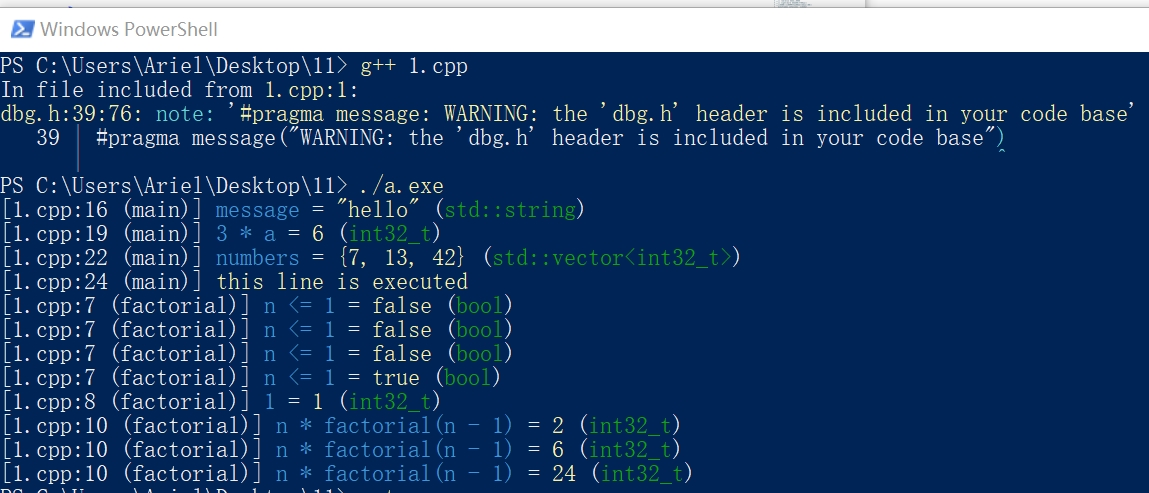
\includegraphics
      [height=.5\textheight]
      {figures/dbg.png}
    \end{stampbox}
    \caption{DBG!}
  \end{figure}
\end{frame}

\makebottom

\end{document}